\newpage
\maketitle


\section{introduction}


What makes mathematics mathematics? 

Recent publications by open AI of math papers demonstrate the potential of LLMs and AI to discover and write proofs. Can a AI practice mathematics for you? I argue there are parts to mathematics that make it inherent to the practiser -- namely the practisers feelings of appreciation and curiosity. On the ladder, a mathemation is in some sense an explorer -- let me make up a world in which these are the rules, and then travel through this world and find out what is true and what isn't. What questions do we care about? It is what questions the mathematition cares about. Maybe an AI can explore aswell, but an AI definitionally cannot explore for you. But maybe AI can be your source of fire as you travel into a cold and unknown rhelm. On the former, we often appreciate beauty. What makes a proof or a theorem beautiful? I often find coorilation between beauty and symmetry. The so called "proof of the other case by simular argument" is something lean cannot do, but is something that can make a proof beautiful, because of its symmetry. Maybe it is abstraction (of which seems to be in coorilation with symmetry aswell) that makes mathematics beautiful. Or, maybe, it is a certain philisophical guideline that is followed in a proof or a theorem or list of axioms. 
In this paper, I try and follow such guideline; namely, that the real numbers are the things you get when you "complete" the rationals, and that the real numbers are themselves sequences of rationals. I don't present anything inherently new, but I try to make what is well studied pretty. I explore what happens when I follow these guidelines, what happens if I use "rational-like" sets instead, and try and abstract my proof to work for completing any metric space. I wish to demonstrate by example that the practise of mathematics carries something very human, at least as human as emotion. 

Given any metric space, you can construct a larger metric space that is complete and contains the original metric space isometrically. Can one do the same to construct the real numbers themselves? How can I construct the real numbers and prove her completeness in a way that emphasizes their cauchy sequence representation, that is simple, beautiful? 


\newpage
%%%%%%%%%%%%%%%%%%%%%%%%%%%%%%%%%%%%%%%%%%%%%%%%%%
%%%%%%%%%%%%%%%%%%%%%%%%%%%%%%%%%%%%%%%%%%%%%%%%%%
\section{Notion of a limit (Review of Topology) }
    % topological
%%%%%%%%%%%%%%%%%%%%%%%%%%%%%%%%%%%%%%%%%%%%%%%%%%
%%%%%%%%%%%%%%%%%%%%%%%%%%%%%%%%%%%%%%%%%%%%%%%%%%


%%%%%%%%%%%%%%%%%%%%%topology%%%%%%%%%%%%%%%%%%%%%%%%%%%%%

\begin{definition} (topology) $\mid$
A \emph{topology} on a set $X$ is a collection $\tau$ of subsets of $X$ (the
\emph{open sets}) such that
\begin{enumerate}[nosep,leftmargin=3em]
    \item $\emptyset \in \tau$ and $X \in \tau$,
    \item any union of members of $\tau$ is in $\tau$,
    \item any finite intersection of members of $\tau$ is in $\tau$.
\end{enumerate}
A \emph{neighborhood} of a point $x$, written $U(x)$, is any open set
containing $x$.
\end{definition}

%%%%%%%%%%%%%%%%%%%%spanning topology%%%%%%%%%%%%%%%%%%%%%%%%%%%%%%

\begin{definition} (spanning topology) $\mid$ \label{def:span}
Say we are given a collection $F\subseteq 2^X$ of subsets of $X$ that we want
to be open. I define the \emph{minimal} (or \emph{generated}, or
\emph{spanning}) topology of $F$ to be
\[
\tau_0(F) := \bigcap \big\{\, \tau \;\big|\; \tau \text{ is a topology on } X
\text{ and } F \subseteq \tau \,\big\}.
\]
Intuitively, $\tau_0(F)$ is what results from applying arbitrary unions and
finite intersections to the members of $F$ and collecting everything so
obtained (hence the name \emph{generated}). Remark~\ref{rem:gen} makes this
precise: one round of finite intersections
followed by one round of unions suffices.
\end{definition}

\begin{lemma} \label{lem:span}
$\tau_0(F)$ is a topology on $X$, it contains $F$, and it is contained in every
topology that contains $F$. So $\tau_0(F)$ is the smallest topology in which
every member of $F$ is open.
\end{lemma}

\begin{remark} (generated = unions of finite intersections) $\mid$ \label{rem:gen}
Let $F^{\cap} := \{B_1\cap\dots\cap B_k \mid k\ge0,\ B_i\in F\}$ (the empty
intersection, $k=0$, is $X$) and $F^{\cap\cup} := \{\text{unions of members of } F^{\cap}\}$
(the empty union is $\emptyset$). Then $\tau_0(F)=F^{\cap\cup}$:
\begin{align*}
&F\subseteq F^{\cap}\subseteq F^{\cap\cup};\qquad \emptyset,X\in F^{\cap\cup};\qquad
\textstyle\bigcup_\beta\bigcup_{\alpha} A_{\beta\alpha}=\bigcup_{\beta,\alpha}A_{\beta\alpha};\qquad
\big(\bigcup_\alpha A_\alpha\big)\cap\big(\bigcup_\beta B_\beta\big)=\bigcup_{\alpha,\beta}(A_\alpha\cap B_\beta)\\
&\qquad\imp F^{\cap\cup} \text{ is a topology containing } F \by{\ref{lem:span}} \tau_0(F)\subseteq F^{\cap\cup}.\\
&\tau\supseteq F \text{ a topology} \imp F^{\cap}\subseteq\tau \imp F^{\cap\cup}\subseteq\tau
\imp F^{\cap\cup}\subseteq\tau_0(F).
\end{align*}
\end{remark}

%%%%%%%%%%%%%%%%%%%%%%basis & its spanning topology%%%%%%%%%%%%%%%%%%%%%%%%%%%%

The definition of $\tau_0(F)$ is abstract: it does not say which sets are open.
When $F$ has two further properties we get a concrete description. This is how
we will understand the metric topology: it is the span of the sets we want to
be open, namely the open metric balls.

\begin{definition} (basis) $\mid$
$F\subseteq 2^X$ is a \emph{basis} if $F$ covers $X$, and whenever
$x \in B_1 \cap B_2$ with $B_1,B_2 \in F$ there is a $B_3 \in F$ with
$x \in B_3 \subseteq B_1 \cap B_2$.
\end{definition}

\begin{theorem} (basis spanning topology) $\mid$ \label{thm:basis}
If $F$ is a basis, then
\[
\tau_0(F) \;=\; \{\, U \subseteq X \mid \forall x \in U,\ \exists B \in F
\mid x \in B \subseteq U \,\} \;=\; \{\text{unions of members of } F\}.
\]
In particular, $U(x)$ is a neighborhood of $x$ in $\tau_0(F)$ exactly when it
contains some $B\in F$ with $x\in B$.
\end{theorem}

%%%%%%%%%%%%%%%%%%order topology%%%%%%%%%%%%%%%%%%%%%%%%%%%%%%%%

\begin{theorem} (order topology) $\mid$ \label{thm:ordertop}
Any totally ordered set $(X,<)$ inherits the following natural topology: the
topology spanned by the basis $\mathcal B$ consisting of $X$ itself, all open
intervals $(a,b)=\{x\mid a<x<b\}$, and all open rays
$(a,\to)=\{x\mid a<x\}$ and $(\leftarrow,b)=\{x\mid x<b\}$.
\end{theorem}

\noindent\textbf{The space $\N\cup\{\infty\}$.} Order $\N\cup\{\infty\}$ by
putting $\infty$ above every natural number, and give it the order topology.

\begin{lemma} \label{lem:infty}
Every neighborhood of $\infty$ in $\N\cup\{\infty\}$ contains a ray
$(N,\to) = \{n\in\N \mid n>N\}\cup\{\infty\}$ for some $N\in\N$. Every such ray
is open, and it contains natural numbers.
\end{lemma}

%%%%%%%%%%%%%%%%%%NOW LIMITS>>>>%%%%%%%%%%%%%%%%%%%%%%%%%%%%%%%%
\bigskip

Next we define limits in general, and then specialize to sequences.
A point $x_0\in X$ is \emph{adherent} to $E\subseteq X$ if every neighborhood
of $x_0$ meets $E$. (Every point of $E$ is adherent to $E$; so is every limit
point of $E$.)

\begin{definition} (limit) $\mid$ \label{def:limit}
Let $X,Y$ be topological spaces, $E\subseteq X$, $f:E\to Y$, and let $x_0\in X$
be adherent to $E$. Then
    \[
    \lim_{\substack{x \to x_0 \\ x \in E}} f(x)
    \text{ exists}
    \iff
    \exists L\in Y \mid
    \forall V(L),\ \exists U(x_0)
    \mid
    f\big(U(x_0)\cap E\big)\subseteq V(L).
    \]
Such an $L$ is called a limit. When $Y$ is Hausdorff (Lemma~\ref{lem:unique})
the limit is unique and we write $L = \lim f(x)$.
\end{definition}

\begin{figure}[H]
\centering
\begin{tikzpicture}

\node[] (X) at (1.75,-1) {};
\node[] at ($(X) + (0,2)$) {$X$};


\draw[blue,thick] (X) ellipse (2 and 2.5);
\begin{scope}[scale=0.5] %% lowkey scale is cutting everything in half, so ... if aint broke don't fix lol
%% E curve
\coordinate (E_start) at (0,0);
\coordinate (C1) at (1,1);
\coordinate (C2) at (7,-3);
\coordinate (E_end) at (5,-5);
\coordinate (C3) at (-1,-4);

\draw[
    thick,
    postaction={decorate},
    decoration={
        markings,
        mark=at position 0.25 with {
            \coordinate (P);
            \fill[red] circle (3pt);
            \draw[red] circle (15pt);
        },
        mark=at position 0.19 with {
            \coordinate (Q);
        },
       mark=at position 0.31 with {
            \coordinate (R);
        }
    }
]
(E_start)
.. controls (C1) and (C2) ..
(E_end)
.. controls (C3) and (E_start) ..
(E_start);

    \end{scope}
    \begin{scope}
    % Only draw inside the red circle
    \clip (P) circle (15pt);

    % A huge hatched region
    \fill[pattern=north east lines]
        ($(Q)$)
        --
        ($(P)$)
        --
        ($(R)$)
        --
        ($(R) + (0,-2)$)
        --
        ($(P) + (0,-5)$)
        --
        ($(Q) + (-1,-2)$)
        -- cycle;

\end{scope}
\node[red,above left=1pt,font=\small] at (P) {$x_0$};
\node[font=\small] at ($(X)+(-1.2,-1.6)$) {$E$};

\coordinate (Y) at ($(X) + (6,0)$);
\draw[] (Y) ellipse (2.5 and 2.5);
\node[] at ($(Y) + (0,2.8)$) {$Y$};


%%%% drawing V(L)
\draw
($(Y) + (0,2)$)
.. controls ($(Y) + (0.75,1.5)$) and ($(Y) + (1.5,1)$) ..
($(Y) + (1.5,0)$)
.. controls ($(Y) + (1.5,-1)$) and ($(Y) + (0.75,0.75)$) ..
($(Y) + (0,-1)$)
.. controls ($(Y) + (-0.75,-0.75)$) and ($(Y) + (-0.75,0.75)$)..
($(Y) + (-0.75,1.8)$)
-- cycle;
\node[font=\small] at ($(Y)+(0.3,1.5)$) {$V(L)$};

%%% drawing f(E \cap U(x_0))
\draw[pattern=north east lines,rotate = 30] ($(Y) + (0.2,0)$) ellipse (0.7 and 0.4);

%%%
\coordinate (L) at ($(Y) + (0.2,0)$);
\fill[red] (L) circle (1pt);
\node[right=0pt] at (L) {$L$};

%%%% the function arrows
% the map itself, between the two spaces
\draw[->,thick] ($(X)+(2.0,1.6)$) -- node[above,font=\small]{$f:E\to Y$} ($(Y)+(-2.1,1.6)$);
% the hatched set U(x_0) \cap E is carried onto the hatched image f(U(x_0) \cap E)
\draw[->,thick,dashed,red!70!black] ($(P)+(0.55,-0.1)$) to[bend right=12]
  node[below,font=\small,pos=0.5]{$f$} ($(L)+(-0.75,0.25)$);

\end{tikzpicture}
\caption{The definition of a limit. Left: the set $E$ (black curve) inside
$X$, the point $x_0$ (red), a neighborhood $U(x_0)$ (red circle) and the
hatched set $U(x_0)\cap E$. Right: a neighborhood $V(L)$ of $L$ in $Y$, which
must contain the hatched image $f(U(x_0)\cap E)$.}
\end{figure}

\begin{definition} (Hausdorff) $\mid$
A topological space $Y$ is \emph{Hausdorff} if any two distinct points
$L\ne L'$ have disjoint neighborhoods $V(L)\cap V(L')=\emptyset$.
\end{definition}

\begin{lemma} (uniqueness of limits) $\mid$ \label{lem:unique}
If $Y$ is Hausdorff, a limit $\lim_{x\to x_0,\,x\in E} f(x)$ is unique when it
exists.
\end{lemma}

\noindent\textbf{Sequential limits.} A sequence in $Y$ is a function
$x:\N\to Y$, $n\mapsto x_n$. By Lemma~\ref{lem:infty}, $\infty$ is adherent to
$E=\N$ inside $X=\N\cup\{\infty\}$, so Definition~\ref{def:limit} applies with
$x_0=\infty$.

\begin{corollary} (sequential limit) $\mid$ \label{cor:seqlim}
For a sequence $x:\N\to Y$,
\[
\lim_{\substack{n \to \infty \\ n \in \N}} x_n = L
\iff
\forall V(L),\ \exists N\in\N \mid \forall n>N,\ x_n \in V(L).
\]
If the topology of $Y$ is spanned by a basis, it is enough to let $V(L)$ range
over basic sets containing $L$.
\end{corollary}

This is the only kind of limit we will need.


%%%%%%%%%%%%%%%%%%%%%%%%%%%%%%%%%%%%%%%%%%%%%%%%%%

%%%%%%%%%%%%%%%%%%%%%%%%%%%%%%%%%%%%%%%%%%%%%%%%%%
%%%%%%%%%%%%%%%%%%%%%%%%%%%%%%%%%%%%%%%%%%%%%%%%%%
\section{Metric Spaces}
%%%%%%%%%%%%%%%%%%%%%%%%%%%%%%%%%%%%%%%%%%%%%%%%%%
%%%%%%%%%%%%%%%%%%%%%%%%%%%%%%%%%%%%%%%%%%%%%%%%%%
%%%%%%%%%%%%%%%%%%%%%%%%%%%%%%%%%%%%%%%%%%%%%%%%%%

We need a more abstract notion of a metric space, since we do not have the
real numbers yet: distances cannot be real numbers. Instead they take values
in a set $V$ in which we can add, subtract and compare. The examples we need
are $V=\Q$ and, later, $V=\Qb$.

\subsection{Well-valued sets}

\begin{definition} (well-valued set) $\mid$ \label{def:wellvalued}
A \emph{well-valued set} is a set $V$ with an operation $+$ and a relation $<$
such that
\begin{enumerate}[nosep,leftmargin=3em,label=(V\arabic*)]
    \item $(V,+)$ is an abelian group (we write $0$ for the identity and
    $-a$ for inverses);
    \item $<$ is a total order satisfying the compatibility implication
    \[ a<b \imp a+c<b+c \qquad\text{for all } a,b,c\in V; \]
    \item $V$ is \emph{Archimedean}: for all $a,b>0$ there exists an
    $n\in\N$ with $na>b$, where $na := a+\cdots+a$ ($n$ times).
\end{enumerate}
I furthermore use the following definitions:
\begin{itemize}[nosep,leftmargin=3em]
  \item $V$ is \emph{dense} if for all $a<b$ in $V$ there is a $c\in V$ with $a<c<b$;
  \item $V$ is \emph{nontrivial} if $V\ne\{0\}$;
  \item $|a| := \max(a,-a)$;\quad $a\le b$ means $a<b$ or $a=b$.
\end{itemize}
\end{definition}
Note: We don't actually need to assume communitivty since (V2) \& (V3) imply it.$ (a + b < (m+n+1) \epsilon, b+a \geq (m+n) \epsilon  \implies a+b - (b+a) < \epsilon $ for all epsilon greater than zero. 

The Archimedean property (V3) is what allows us to build a sequence tending to
zero (Lemma~\ref{lem:nullseq}). Actually, for the completeness proofs we only
need the \emph{existence} of such a sequence; but with only that assumption we
can end up constructing things that are not $\R$. This is still interesting,
and we come back to it in Section~\ref{sec:nullseq}.

\begin{remark} (positivity) $\mid$ \label{rem:pos}
Given (V1), condition (V2) is equivalent to a notion of \emph{positivity}: a
set $P\subseteq V$ (the positive elements) with
\[
\text{(P1)}\ \ P+P\subseteq P,
\qquad
\text{(P2)}\ \ \forall a\in V \text{ exactly one of } a\in P,\ a=0,\ -a\in P.
\]
\begin{align*}
&\text{(V2)}\Rightarrow\text{(P)}:\quad P:=\{a\mid a>0\}.\qquad
a,b>0 \imp a+b>0+b=b>0\ \ \text{(P1)};\\
&\qquad\qquad\qquad\ \ a>0 \iff 0>-a\ \ (\text{add } -a),\ \text{so (P2) is totality of } <.\\[3pt]
&\text{(P)}\Rightarrow\text{(V2)}:\quad a<b \ :\iff\ b-a\in P.\qquad
c-a=(c-b)+(b-a)\ \ \text{(transitive)};\\
&\qquad\qquad\qquad\ \ \text{(P2)}\ \ \text{(total)};\qquad (b+c)-(a+c)=b-a\ \ \text{(compatible)}.
\end{align*}
This is how we will put an order on $\Qb$.
\end{remark}

\begin{lemma} (arithmetic of inequalities) $\mid$ \label{lem:ineq}
In a set satisfying (V1) and (V2):
\begin{enumerate}[nosep,leftmargin=3em]
    \item[(a)] $a<b,\ c\le d \imp a+c<b+d$;
    \item[(b)] $a<b\iff -b<-a$;
    \item[(c)] $|a|\ge0$;\ \ $|a|=0\iff a=0$;\ \ $|-a|=|a|$;\ \ $|a+b|\le|a|+|b|$;\ \
    $\big||a|-|b|\big|\le|a-b|$;
    \item[(d)] for $n\ge1$: $na<nb\iff a<b$.
\end{enumerate}
\end{lemma}

\begin{lemma} (halving) $\mid$ \label{lem:halving}
If $V$ is dense: $\ \epsilon>0 \imp \exists\eta>0$ with $\eta+\eta\le\epsilon$.
\end{lemma}

\noindent\textbf{Notation.} For $\epsilon>0$ in a dense $V$ we write
$\epsilon/2$ for an element $\eta>0$ as in Lemma~\ref{lem:halving}, and
$\epsilon/4$ for $(\epsilon/2)/2$, so $4(\epsilon/4)\le\epsilon$; we write
$\epsilon/3$ for $\epsilon/4$, which satisfies $3(\epsilon/3)<\epsilon$. When
$V=\Q$ these are literally $\epsilon/2$, $\epsilon/4$ and (one may take)
$\epsilon/3$. All we ever use is
\[
\epsilon/2+\epsilon/2\le\epsilon,\qquad
3(\epsilon/3)\le\epsilon,\qquad
4(\epsilon/4)\le\epsilon,\qquad
0<\epsilon/2<\epsilon,\qquad
\epsilon-\epsilon/2\ge\epsilon/2 .
\]

%%%%%%%%%%%%%%%%%%%%%%%%%%%%%%%%%%%%%%%%%%%%%%%%%%%
%%%%%%%%%%%%%%%%%%%%%%%%%%%%%%%%%%%%%%%%%%%%%%%%%%%

\subsection{Metric spaces and the metric topology}

\begin{definition} (metric space) $\mid$
Let $V$ be a nontrivial set satisfying (V1) and (V2). A \emph{metric space}
with values in $V$ is a set $X$ with a function $d:X\times X\to V$ such that
for all $x,y,z\in X$:
\begin{enumerate}[nosep,leftmargin=3em]
    \item $d(x,y)\ge 0$, and $d(x,y)=0 \iff x=y$,
    \item $d(x,y)=d(y,x)$,
    \item $d(x,z)\le d(x,y)+d(y,z)$ (triangle inequality).
\end{enumerate}
The \emph{open ball} of radius $\epsilon\in V$, $\epsilon>0$, is
$B_\epsilon(x) = \{y\in X \mid d(x,y)<\epsilon\}$.
\end{definition}

\begin{lemma} (metric topology) $\mid$ \label{lem:metrictop}
The open balls form a basis. The topology they span, the \emph{metric
topology}, is
\[
\{\,U\subseteq X \mid \forall x\in U,\ \exists\epsilon>0 \mid
B_\epsilon(x)\subseteq U\,\},
\]
which is the usual definition of an open set. Consequently, for sequences, (for the case of dense V, use triangle inequality to show, given an open ball containing L, we can make a open ball centered at L contained in the former ball. For the non-dense V, the sequence must be eventaully constant so the definitions coincide.)
\[
\lim_{n\to\infty} x_n = L
\iff
\forall \epsilon\in V,\ \epsilon>0,\ \exists N \mid \forall n>N,\ d(x_n,L)<\epsilon .
\]
\end{lemma}

We write $d\text{-}\lim$ when we want to name the metric being used.

\begin{lemma} (metric spaces are Hausdorff) $\mid$ \label{lem:hausdorff}
Let $V$  Every metric space with values in $V$ is Hausdorff. Hence
limits in such spaces are unique (Lemma~\ref{lem:unique}). (treat each case separately: V is dense, V is not dense \& non-trivial, V is trivial)
\end{lemma}

\begin{definition} (natural metric of a well-valued set) $\mid$ \label{def:natmetric}
Any well-valued set $V$ inherits the following natural metric, with values in
$V$ itself:
\[
d:V\times V\to V,\qquad d(x,y)=|x-y| .
\]
\end{definition}

\begin{lemma} \label{lem:natmetric}
$d(x,y)=|x-y|$ is a metric on $V$, and its metric topology is the order
topology of Theorem~\ref{thm:ordertop}.
\end{lemma}

%%%%%%%%%%%%%%%%%%%%%%%%%%%%%%%%%%%%%%%%%%%%%%%%%%%
%%%%%%%%%%%%%%%%%%%%%%%%%%%%%%%%%%%%%%%%%%%%%%%%%%%

\subsection{Cauchy sequences and holes}

\begin{definition} (Cauchy sequence, completeness) $\mid$
A sequence $(x_n)$ in a metric space $(X,d)$ is \emph{Cauchy} if
\[
\forall \epsilon>0,\ \exists N \mid \forall n>N,\ d(x_n,x_N)<\epsilon.
\]
$(X,d)$ is \emph{complete} if every Cauchy sequence in $X$ converges to a
point of $X$.
\end{definition}


\begin{figure}[H]
\centering
\begin{tikzpicture}[x=1.0cm,y=1cm]
  % Points only, no horizontal line
  \foreach \x/\lab in {
    0/{x_1},
    1.2/{x_2},
    2.4/{x_3},
    3.6/{x_4},
    4.8/{\cdots},
    6.0/{x_N},
    9.0/{x_n},
    10.5/{x_m},
    11.7/{\cdots}
  }{
    \fill (\x,0) circle (1.8pt);
    \node[below,font=\small] at (\x,-0.05) {$\lab$};
  }

  % Curved arrows pointing toward x_N
  \draw[->,thick]
    (9.0,0.08)
    .. controls (8.8,1.0) and (6.8,1.0) ..
    node[midway,above,font=\small] {$<\epsilon$}
    (6.08,0.12);

  \draw[->,thick]
    (10.5,0.08)
    .. controls (10.2,1.8) and (7.0,1.8) ..
    node[midway,above,font=\small] {$<\epsilon$}
    (6.08,0.12);

\end{tikzpicture}
\caption{The Cauchy condition: all sufficiently late terms lie within
$\epsilon$ of the fixed term $x_N$.}
\label{fig:cauchy}
\end{figure}

This is how the condition is used in proofs: to compare two late terms
$x_n,x_m$ we move each of them to $x_N$,
$d(x_n,x_m)\le d(x_n,x_N)+d(x_N,x_m)<\epsilon+\epsilon$, so we only ever
measure distances to this one $x_N$ (Figure~\ref{fig:cauchy2}).

\begin{lemma} (convergent $\Rightarrow$ Cauchy) $\mid$ \label{lem:convcauchy}
Let $V$ Every convergent sequence is Cauchy.
\end{lemma}

\begin{lemma} (Cauchy sequences are bounded) $\mid$ \label{lem:bounded}
$(x_n)$ Cauchy $\imp \exists a\in X,\ M\in V:\ \forall n,\ d(x_n,a)\le M$.
\end{lemma}

A \emph{hole} is the failure of the converse of Lemma~\ref{lem:convcauchy}:
a Cauchy sequence that tries to converge but has nothing in the space to
converge to. Every Cauchy sequence is bounded (Lemma~\ref{lem:bounded}), and
much more is true: for each $\epsilon$ its whole tail beyond some $N$ is
squeezed inside the ball $B_\epsilon(x_N)=(x_N-\epsilon,\,x_N+\epsilon)$, and
we may make $\epsilon$ as small as we like. So the tail is trapped in smaller
and smaller balls, and any Cauchy sequence seems to ``converge'' to something.
When it does not, the place it is squeezing down on is missing from the
space, and we call it a \emph{hole} (Figure~\ref{fig:hole}).

\begin{figure}[ht]
\centering
\resizebox{\textwidth}{!}{%
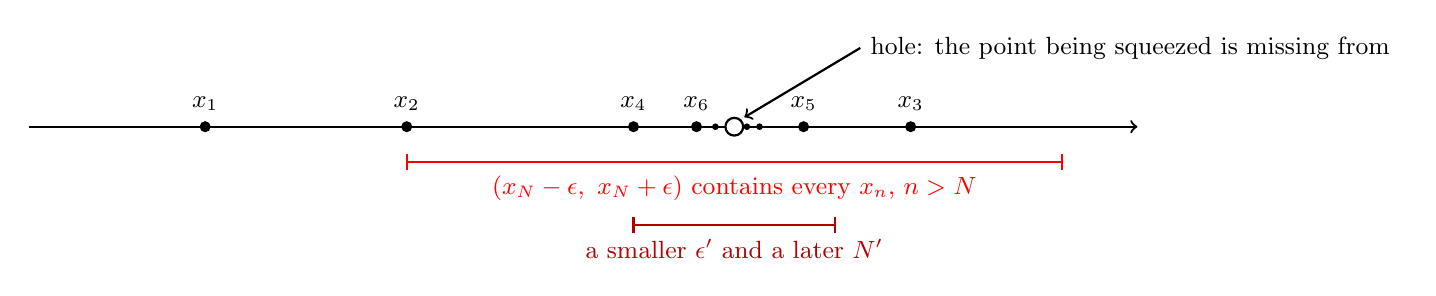
\begin{tikzpicture}[x=1.6cm]
% the line Q with a hole
\draw[thick,->] (-0.4,0) -- (8.4,0) node[right]{$\Q$};
\coordinate (H) at (5.2,0);
% the terms of the sequence, squeezing down on H
\foreach \x/\lab in {1/{x_1},2.6/{x_2},6.6/{x_3},4.4/{x_4},5.75/{x_5},4.9/{x_6}}{
  \fill (\x,0) circle (2pt);
  \node[above,font=\small] at (\x,0.08) {$\lab$};
}
\foreach \x in {5.4,5.05,5.3,5.15,5.24,5.18}{
  \fill (\x,0) circle (1.2pt);
}
% nested squeezing intervals
\draw[red,thick] (2.6,-0.45) -- (7.8,-0.45);
\draw[red,thick] (2.6,-0.35) -- (2.6,-0.55);
\draw[red,thick] (7.8,-0.35) -- (7.8,-0.55);
\node[red,font=\small,below] at (5.2,-0.5) {$(x_N-\epsilon,\ x_N+\epsilon)$ contains every $x_n$, $n>N$};
\draw[red!70!black,thick] (4.4,-1.25) -- (6.0,-1.25);
\draw[red!70!black,thick] (4.4,-1.15) -- (4.4,-1.35);
\draw[red!70!black,thick] (6.0,-1.15) -- (6.0,-1.35);
\node[red!70!black,font=\small,below] at (5.2,-1.3) {a smaller $\epsilon'$ and a later $N'$};
% the hole
\draw[thick,fill=white] (H) circle (3.2pt);
\draw[->,thick] (6.2,1.0) node[right,font=\small]{hole: the point being squeezed is missing from $\Q$} -- (5.28,0.12);
\end{tikzpicture}%
}
\caption{A hole. The terms of a Cauchy sequence get trapped in smaller and
smaller intervals (red). They squeeze down on a single location, but if that
location (open circle) is not a point of the space, the sequence has nothing
to converge to.}
\label{fig:hole}
\end{figure}

There exist well-valued sets with holes!

\begin{theorem} (Q has holes) $\mid$ \label{thm:holes}
The rational numbers with their natural metric $d(x,y)=|x-y|$ are not
complete.
\end{theorem}

\begin{lemma} (non-dense well-valued sets have no holes) $\mid$
\label{lem:nondense}
This is trivially true in the trivial case since the ambient space can only have one element. So, let $V$ be a nontrivial well-valued set that is \emph{not} dense. Then $V$ has
a smallest positive element $p$, $V=\{kp\mid k\in\Z\}$ is a copy of the
integers, and every metric space with values in $V$ is complete.
\end{lemma}

Henceforth we are only concerned with dense well-valued sets; by
Lemma~\ref{lem:nondense} nothing is lost. Such sets I like to call
\emph{$\Q$-like}. The goal is to construct a completion of these sets. 

(In looking for simular uses of such well-valued sets, I note Hölders theorem which says any such well valued set is a subgroup of the reals. Such a result is a simple implication of the results of the completeness proof of this paper with lemma \ref{lem:nondense} In essense we have already considered the simple cases of when V is not dense or trivial... now we consider the interesting case...)

\begin{definition} ($\Q$-like set) $\mid$ \label{def:qlike}
A \emph{$\Q$-like set} is a dense, nontrivial well-valued set.
\end{definition}

%%%%%%%%%%%%%%%%%%%%%%%%%%%%%
% properties of Q-like sets:
%   - halving (Lemma halving, above)
%   - sequence to zero
%%%%%%%%%%%%%%%%%%%%%%%%%%%%%

\begin{lemma} (a sequence tending to zero) $\mid$ \label{lem:nullseq}
Let $V$ be $\Q$-like. There is a sequence $(e_n)$ in $V$ with
\[
e_n>0,\qquad e_{n+1}+e_{n+1}\le e_n,\qquad
\forall\epsilon>0\ \exists N\ \forall n\ge N,\ e_n<\epsilon .
\]
(such a sequence looks like $e_n=(\frac12)^n$.)
\end{lemma}